%Use graph with 
\chapter{Methods and Set-Up}
\label{sec:methods}
\section{Perturbation Scheme}
\begin{figure}
    \centering
    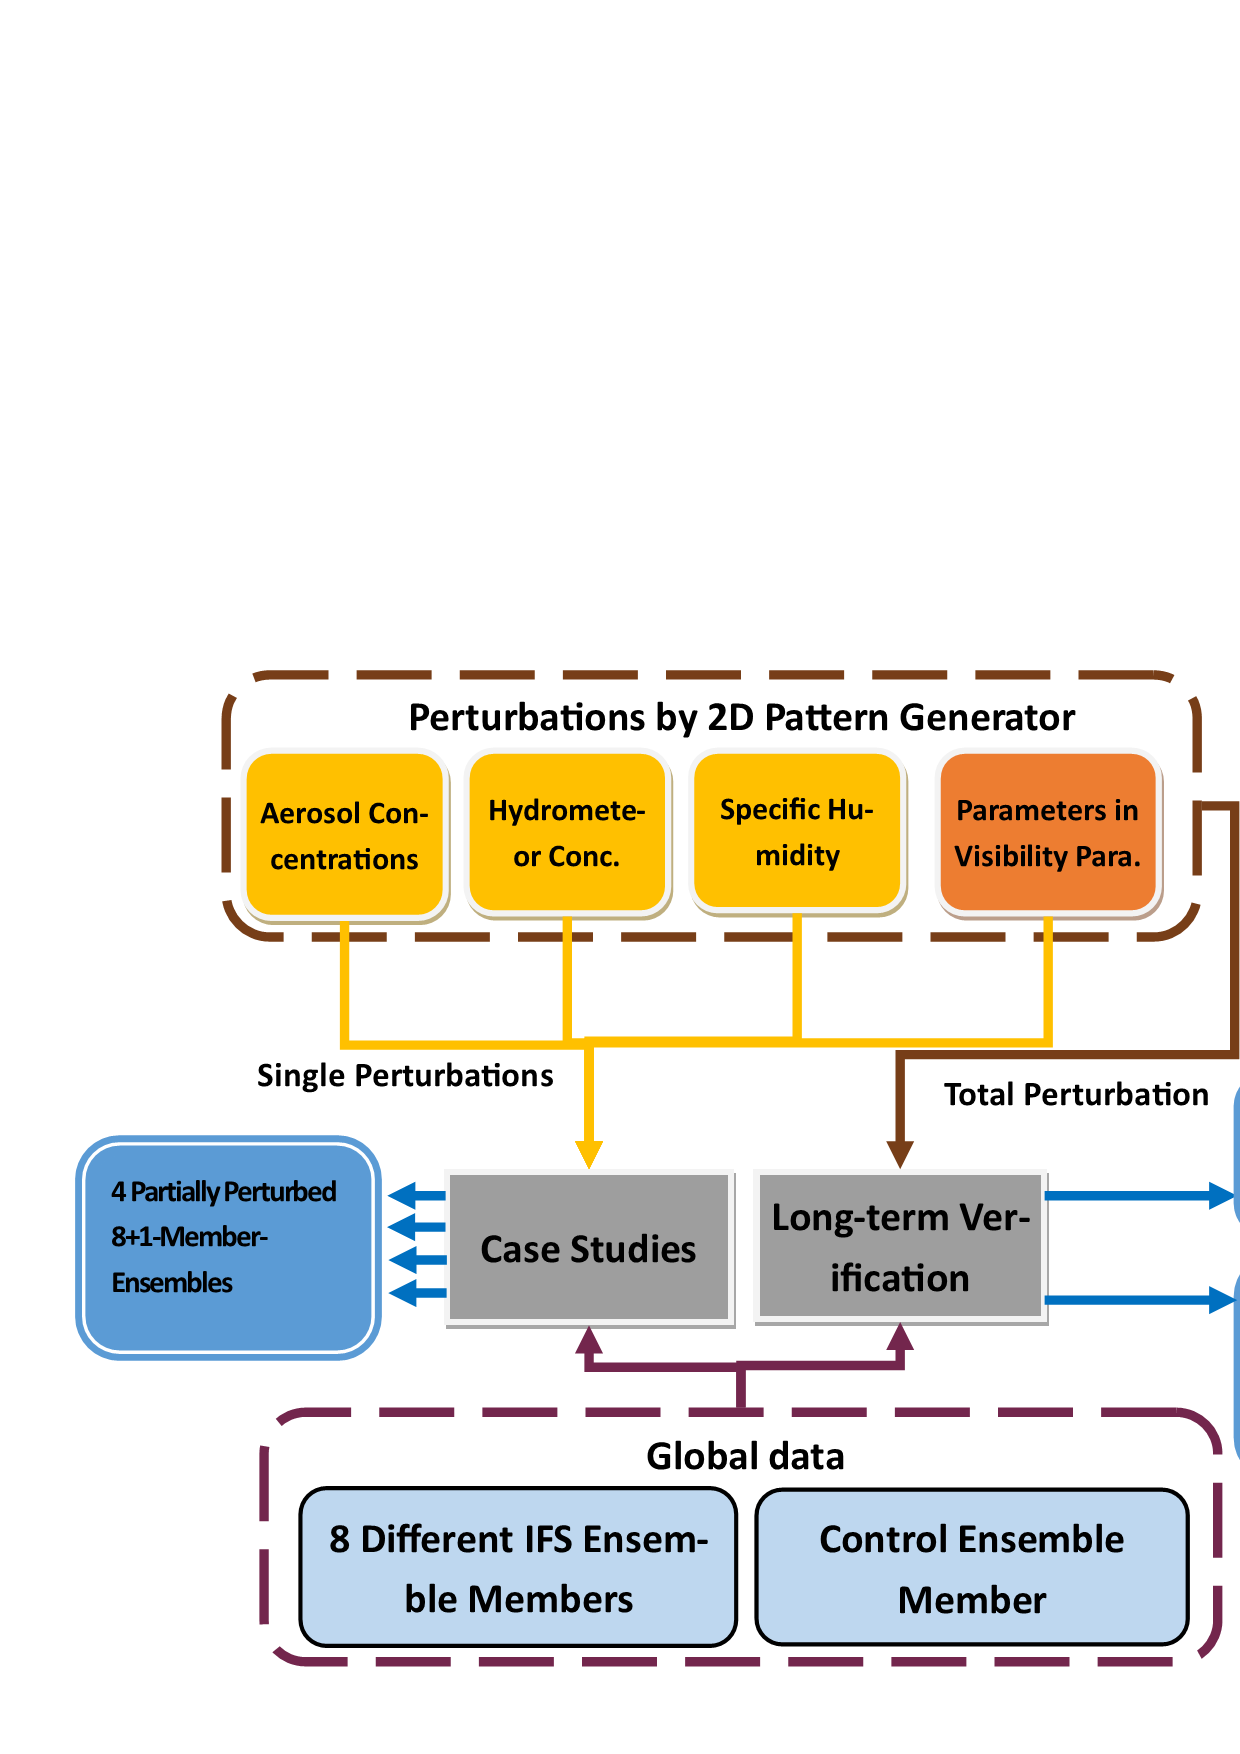
\includegraphics[width=\textwidth]{graphics/Perturbationsscheme.png}
    \caption[Illustration of Perturbation Scheme]{Illustration of the perturbation scheme: Showing the different perturbed quantities at the top and the used ensemble members from the IFS model on bottom. }
    \label{fig:pertrubation_scheme}
\end{figure}
For the evaluation of the parametrization, several forecasts with different perturbation schemes, also called NWP experiments, were performed.
To investigate the influence of different variables on visibility, the following versions of perturbations, presented in Figure \ref{fig:pertrubation_scheme}, were tested:
\begin{enumerate}
    \item{Control ensemble}
    \item {Perturbation of aerosol concentrations}
    \item {Perturbation of hydrometeors}
    \item {Perturbation of the parameters in the visibility parametrization}
    \item {Perturbation of specific humidity}
    \item {Total perturbation (aerosols, hydrometeors, specific humidity, parameters) }
    
\end{enumerate}
Figure \ref{fig:pertrubation_scheme} illustrates the listed perturbed variables and which combinations were run as case studies and for the long-term verification. No additional perturbation was applied to the control ensemble. It constitutes of an AROME ensemble, which was created by using data of eight perturbed members and one control member of the IFS ensemble to set different boundary and initial conditions for each member. The measured visibility lies often outside the ensemble spread of the control ensemble, mainly, because this ensemble does not take model error into account. Especially for visibility, many of the key parameters are hard to predict reliably and often not varied in the standard perturbation schemes \cite{chmielecki2011probabilistic}. To tackle this underdispersion of the control ensemble, additional local perturbations were introduced.\\
In this case, local means, the perturbations were chosen and set-up to be applied only in the visibility module. The other parts of the model remained untouched. \\
For the perturbed ensemble, the current values are perturbed with the corresponding spatial-temporal pattern  at each time step and the perturbed quantities are passed on to the visibility parametrization and thus, do not affect any future states of the model. This method forbids the perturbations to be amplified in time, and therefore the default amplitudes must be higher in comparison to a perturbation scheme that is applied to the overall model and can evolve.
The reason why a local perturbation scheme is used, is that no global perturbation scheme for AROME is available, where all the relevant parameters and variables can be perturbed.
Perturbing all of them globally, would lead to a change in a number of non-linear feedback processes. The model could not handle those perturbations, because the effects of different perturbations can have conflicting outcomes for different variables. Since we are only interested in investigating the uncertainty of the visibility forecast, a local perturbation is sufficient.\\
Although we can estimate the ranges for all parameters quite well, we have very little a priori knowledge about the compatibility of the values of different variables after a certain time.\\
For a locally applied perturbation, the distance to the original trajectory in phase space can be restricted and chosen small enough to have tolerable errors. If we would allow them to propagate, we are unable to predict how the perturbed trajectory will evolve. There is no guarantee that it will lead to a realistic outcome at a later time, because the tolerable error can be amplified to a completely nonsensical scenario. 
There are several other attempts of probabilistic forecasting of visibility \cite{chmielecki2011probabilistic, Roquelaure}, but we believe that the advantage of our method is its comprehensible nature. It is not purely statistical but relates to single physical quantities.\\

The details of the perturbation scheme are outlined in the following subsections.
%Aufzehulgn jeder ienzelnen Storung und Beschreibung der range einschraenkung

\subsection{Set-Up of Perturbations}
All perturbations were generated by use of the pattern generator described in Section \ref{sec:pattern gen}. The spatial correlation length was only roughly estimated in terms of large-scale and meso-scale processes, because it, is only a namelist setting and has a complex relation to the actual spatial scale. It cannot be directly related to a length scale, because it is scaled with respect to the Earth's radius, since it was originally set-up for a global model. All fields, with exception of the aerosol concentrations, are assumed to be meso-scale perturbations. Temporal correlations were all set to 72 hours, because the time scales have a negligible impact, since the local perturbations cannot evolve in time.\\
A weakness of the implementation of the pattern generator is that when multiple fields are perturbed that perturbations can vary in spatial and temporal correlation length, but all of them must have the same clip ratio $x_{\mathrm{clip}}$, which was set to 1. Same holds for $\sigma_{\mathrm{nl}}$, which was set to 0.05.\\
To compensate for this, we introduced scaling factors that are applied to the perturbations in the appropriate way. They are different for each quantity and explained later in this section, when the details of the perturbations for each quantity are provided.\\
Depending on the perturbed quantity and the perturbation scheme, we needed to define a suitable range for each quantity, implemented by means of the scaling factor.\\
For some quantities, like the aerosol concentrations, global data and its extrema can be used (see Table \ref{tab:ensem}) to determine the range.
In other cases there are no global extrema to be considered, but a physical constraint, like a quantity being greater than zero (e.g. the surface-volume-coefficients). If the related phenomena are strongly local, like precipitation, local climatological extrema are appropriate gauge values for the perturbation ranges.
The different constituents of the perturbation scheme are presented in Table \ref{tab:ensem} with the corresponding restriction of the perturbation range.
Table \ref{tab:ensem} shows all considered uncertainties of the scheme and the type of the errors, where the uncertainties originate from. It provides an overview of the different restrictions of the quantities, which limit the ranges and are discussed in the following.

\begin{table}[h]
\captionsetup{justification=justified}

    \footnotesize
    \centering
        \begin{tabular}{|l|c|c|}
        \hline
        \textbf{Contributor}&\textbf{Restrictions}&\textbf{Type}  \\
        \hline
        \hline
        IFS Global Model&8 Members& b.c.s/i.c.s *\\
        \hline
        Specific Humidity & 10\% of $q_{\mathrm{spec}}$&Model Error\\
        \hline
        Hydrometeors&Local Climatological Extrema&Model Error \\
        \hline
        Aerosols&Global Climatological Extrema&Model Error \\
        \hline
        $c_{i}$ in the $vis$ parametrization&Physical Considerations&Model Error\\
        \hline
    \end{tabular}
    \caption{\footnotesize{Constituents of the Perturbation Scheme: Different contributors differ in the source of error and the restrictions for the ranges.\\ \tiny{*b.c.s=boundary conditions; i.c.s=initial conditions} }}
    \label{tab:ensem}
\end{table}
The namelist settings for the pattern generator for each field or variable can be found in Table \ref{tab:namelist_pert} in Appendix \ref{sec:tabelappendix}.


\subsubsection{Perturbation of IFS data}
The control ensemble is created in AROME by using eight different members and the control member of the global IFS model. The IFS-ensemble provides different initial and boundary conditions, that were gained by the application of the ECMWF perturbation scheme documented in \cite{documentationpart} and \cite{IFS}. In all other perturbation regimes the perturbation is applied in addition to the varying  initial and boundary conditions taken from the IFS.

\subsubsection{Perturbation of Hydrometeors}
When analysing the uncertainty of hydrometeor concentration, we find two contributors: the location of the hydrometeors and the actual concentrations.\\
The discrepancy of model and reality is considered worse, when on certain locations no occurrence of hydrometeors is forecast, but in reality some clouds, or precipitation are reported, than in comparison of wrong estimation of precipitation just in terms of heaviness.
Hence, the perturbation scheme has to include variance in location in a way, that also on locations where the unperturbed fields of the concentrations are zero, they can be non-zero on the perturbed fields.
The tendencies of the hydrometer concentrations were used to create such a perturbation scheme that also relates to the current weather situation, by using the accumulated tendencies from previous time steps.\\
To understand the perturbation regime, one has to understand the calculation of the unperturbed hydrometeor concentrations 
\begin{equation}
    c_{i}(t_{n}) = c_{i}(t_{n-1}) + T_{c_{i}}(t_{n})
    \label{eq:hydro}
\end{equation}
first. The concentration $c_{i}$ at a time $t_{n}$ is the sum of the concentration at the previous time step of the hydrometeor $c_{i}(t_{n-1})$ and the tendency of the concentration of the hydrometeor $T_{c_{i}}$ at $t_{n}$. The tendency $T_{c_{i}}$ is the sum of the output of different physical parametrizations. These parametrizations take other model variables (at the current time step) as input, e.g. humidity and temperature, so that hydrometeor concentration and distribution are related to the updated overall atmospheric state.\\ \\
The perturbations $P_{c_{i}}$ are set up as the past accumulated tendencies multiplied by the exponential of a random number $r_{j}$ summed up over a time span $t_{\mathrm{acc}}$. For this study the time span is set to two hours.
\begin{equation}
    P_{c_{i}}(t_{\mathrm{N}}) = \sum\limits_{t_{n}=t_{\mathrm{N}}-t_{\mathrm{acc}}}^{t_{\mathrm{N}}} T_{c_{i}}(t_{n})\exp(r_{j})
    \label{eq:}
\end{equation}
As described by Equation \eqref{eq:petconhyd}, the perturbed concentration $\tilde{c}_{i}(t_{n})$ is set by adding the perturbation to the unperturbed quantity $c_{i}(t_{n})$.
\begin{equation}
    \tilde{c}_{i}(t_{n}) = c_{i}(t_{n}) + sP_{c_{i}}(t_{n})
    \label{eq:petconhyd}
\end{equation}
The perturbation is scaled by the factor $s$. The scaling factor $s$ was gained by testing different values under the criterion, that the perturbed concentrations cannot exceed the doubled monthly extrema on the domain $L$. This restrain was chosen, because the climatological data is a good reference in terms of what can be considered as in the norm. Global extrema are irrelevant, since precipitation depends strongly on the climate zone. The advantage of using the tendencies of a time span, close to the current time, is that the change in location of the hydrometeors is related to local weather conditions that promote the presence of hydrometeors. 

\subsubsection{Perturbation of Aerosols}
Aerosol distributions are usually evolving on a global scale \cite{tegen1997contribution,chin1996global, liousse1996global,tegen1995contribution}. Hence, it is reasonable to use global extrema to set the ranges for the perturbed aerosol concentrations $ \tilde{c}_{j}$ on the LAM domain. To do so, some general considerations about local and global extrema in NWP and stochastic physics ensembles are made:\\
When the unperturbed quantity $\xi$, in a LAM has a local maximum $\mathrm{max_{local}}$ and local minimum $\mathrm{min_{local}}$ on a local domain $L$, the perturbation range must be chosen in a way, that the perturbed quantity $\tilde{\xi}$ cannot exceed any known global extrema $\mathrm{max_{global}}$ or $\mathrm{min_{global}}$.
To make sure that the perturbed quantity $\tilde{\xi}$ is in a physically reasonable range on $L$ for any possible case, the following condition must hold at all times:
\begin{equation}
\mathrm{min_{global}} < \tilde{\xi} < \mathrm{max_{global}}.
\label{rangecrit}
\end{equation}

This leads to the criteria for the range $a$ for log-normally distributed perturbations:
\begin{equation}
a_{\mathrm{log}}(\mathrm{max}) = \ln \left( \frac{\mathrm{max_{global}}}{\mathrm{max_{local}}} \right)
\label{eq:logmax}
\end{equation}

\begin{equation}
a_{\mathrm{log}}(\mathrm{min}) = \ln \left( \frac{\mathrm{min_{local}}}{\mathrm{min_{global}}} \right)
\end{equation}

Since in most cases the range criteria vary, depending on choosing a restriction with respect to minimum or maximum, one has to decide, if one extremum can be used and the other one be exceeded or not even reached.\\
We decided to set the range with respect to the maximum. Thus, the global minimum is not reached, because the amplitude of the perturbation is too small. This is justified by the greater importance of the maximum for a realistic estimate of the worst case scenario of the lowest possible visibility.\\

The aerosols concentrations $c_{j}$ are perturbed by multiplying the concentration by an exponential function: 
\begin{equation}
    \tilde{c}_{j} = c_{j} \ \exp(sr_{j})  \quad .
    \label{eq:aerpert}
\end{equation}
The scaling factor $s$ was calculated for each aerosol as described by Equation \eqref{eq:logmax} and all values are presented in Table \ref{tab:scale_aerosol} in Appendix \ref{sec:tabelappendix}. \\
Because the climatological aerosol data varies monthly \cite{nasa}, the scaling factor was calculated for each month. Because the dynamics of aerosols happens on larger scales than most other atmospheric transport processes and by investigation of the global aerosol data set \cite{nasa}, the spatial correlation length for the pattern generator was estimated to be 200000km. It is important to keep in mind that this correlation length does not correspond directly to the scale of the process but in a complex non-linear manner as described in Section \ref{sec:pattern gen}.

\subsubsection{Perturbation of Physical Parameters}
The surface-volume-coefficients of hydrometeors, scattering cross sections and  mass attenuation coefficients of aerosols were perturbed. The motivation is that these parameters were set to one `best-guess' value, but in reality  they depend on the radii of the particles, which can vary significantly. The extinction caused by Rayleigh scattering is also perturbed because the changes in distributions of the composition of the gaseous components of air are neglected in the model. All these physical parameters need to be greater than zero at all times. Additionally, the physical assumptions for different relevant processes in the related works of \citeauthor{stoelinga1999nonhydrostatic} \cite{stoelinga1999nonhydrostatic} and \citeauthor{tegen1997contribution} \cite{tegen1997contribution} were used as well as the set-up of the ECMWF stochastic physics scheme described by \citeauthor{ollinaho2017towards} \cite{ollinaho2017towards}. Then test cases were run to study the impact of the perturbations and empirically adapt the perturbations to the values presented in Table \ref{tab:namelist_pert} in Appendix \ref{sec:tabelappendix}. 
\subsubsection{Perturbation of Specific Humidity}
 The works of \citeauthor{Stensrud} \cite{Stensrud} was used as a point of reference to set the range for specific humidity. \citeauthor{Stensrud} provide statistics about the RMSE values, which let us estimate an initial perturbation of 10\%. Then, again, test cases were run to study the impact of the perturbations and empirically adapt the perturbations to their final values presented in Table \ref{tab:namelist_pert} in Appendix \ref{sec:tabelappendix}. 

\section{Set-Up}

\begin{table}[h]
    \footnotesize
    \centering
    \begin{tabular}{|l|c|c|}
        \hline
        \rule{0pt}{16pt}{\large \textbf{Model Setting}}&{\large \textbf{Value}}&{\large \textbf{Effect} }\\ 
        \hline
        \hline
        \textbf{Lag Time}&36h&Total Spread\\
        \hline
        \textbf{Coupling Frequency}&3h&Dependence on Global Model\\
        \hline
        \textbf{Forecast Duration}&18h&Available Outputs, Total Spread\\
        \hline
        \textbf{Base Time}&00:00&Available Outputs, Total Spread\\
        \hline
        \textbf{Long Term Verification}&July 2016&Evaluation\\
         &January 2017&\\
        \hline
        \textbf{Case Studies} &10.07.2016&Impacts of Single Quantities\\
        & 14.07.2016&\\
        &08.01.2017&\\
        &21.01.2017&\\
        &29.01.2017&\\
        \hline
    \end{tabular}
    \caption{Overview of the model's settings, the chosen verification periods and case studies.}
    \label{tab:modelparam}
\end{table}

The model output was created from the totally perturbed ensemble, which incorporates all single perturbations, and the control ensemble for two whole months to obtain a large enough data set for the verification process.
The months January 2017 and July 2016 were chosen, to be able to analyse data of summer and winter conditions.
In addition, all the different versions of single perturbations were run for the following selected dates: \textbf{10.07.2016, 14.07.2016, 08.01.2017, 21.01.2017, 29.01.2017}.\\
The days for the case studies were selected with having in mind, the want of investigating a broad variation of weather conditions. The case studies are of great importance to gain a deeper insight into the impact of each parameter and variable.\\ \\
Since the overall ensemble spread is known to be too low, the model settings presented in Table \ref{tab:modelparam} are chosen under the aspect of amplifying it.\\
The \textbf{base time}, which denotes the starting time of a forecast, was set to \textbf{00:00 UTC} and the \textbf{forecast duration to 18 hours}. UTC stands for Universal Time, Coordinated and means that only one global time zone is used. The setting was chosen, because visibility measurements are taken from 06:00 to 18:00 UTC. A base time of 00:00 UTC assures that the ensemble can evolve before the first value for verification is taken.
For every run eight randomly selected ensemble members from the global IFS ensemble were taken, to investigate the effect of varying initial conditions. This number was chosen based upon what is computationally affordable and still gives a reasonable spread \cite{buizza1998impact}.
For each member a different perturbation pattern was applied, by passing on a different seed to the random number generator. In addition every parameter has a different pattern.
The purpose of this is to model the realistic scenario that different components in a system can either amplify or damp one and another.\\


The coupling of the global and the limited area model is something that has great influence on the model spread. The lag time is the parameter that defines the difference of the base time of the run of the global model and the base time of the limited area model. It is known that for short-range and medium-range forecasts on average, the longer a forecast period lasts, the higher the spread is \cite{buizzaskillspread, bauer2015quiet}. Hence, the lag time has an impact, because if we take different ensemble members after a long forecast period the initial conditions have a much higher variation, than if they were taken at an earlier stage. We set the \textbf{lag time to 36 hours}.
The coupling frequency is the model parameter that determines how often the boundary conditions should be updated with respect to the global model. The coupling is especially important, to avoid that the limited area model can evolve over longer periods of time in a way that is in total disagreement with the global model, and hence nonsensical.
So the best is to couple as often as possible, with regards to availability of global data and computational affordability. For this study the \textbf{coupling frequency is set to three hours}.
